\documentclass[12pt,a4paper]{article}

% Packages
\usepackage[utf8]{inputenc}
\usepackage[english]{babel}
\usepackage{amsmath}
\usepackage{amssymb}
\usepackage{amsthm}
\usepackage{graphicx}
\usepackage{booktabs}
\usepackage{multirow}
\usepackage{longtable}
\usepackage{caption}
\usepackage{subcaption}
\usepackage{float}
\usepackage{geometry}
\usepackage{setspace}
\usepackage{hyperref}
\usepackage{natbib}
\usepackage{enumitem}

% Page layout
\geometry{
    top=1in,
    bottom=1in,
    left=1in,
    right=1in
}

% Line spacing
\onehalfspacing

% Hyperref setup
\hypersetup{
    colorlinks=true,
    linkcolor=blue,
    citecolor=blue,
    urlcolor=blue
}

% Title and author
\title{\textbf{The Impact of Major Game Patches on Player Engagement:} \\ A Difference-in-Differences Analysis of Steam Games}
\author{Your Name Here}
\date{\today}

\begin{document}

\maketitle

\begin{abstract}
This study examines whether major game patches causally affect player engagement in Steam games. Using difference-in-differences methodology with two complementary designs---a staggered DiD analysis (320 games, 5 months) and a February 2025 single-cohort analysis (145 games, 4 weeks)---we find that major patches increase average concurrent players by approximately 6\% ($p=0.044$). We document substantial selection bias in naive comparisons, with pooled OLS models overestimating effects by 35 percentage points. Our preferred two-way fixed effects specification controls for time-invariant game characteristics and aggregate time shocks, providing credible causal estimates. Results are robust across different treatment timings and model specifications. These findings suggest that while major patches do increase player engagement, the effect is modest and developers should maintain realistic expectations about patch impacts.

\noindent \textbf{Keywords:} Video games, Difference-in-Differences, Causal inference, Player engagement, Steam platform, Game patches
\end{abstract}

\newpage
\tableofcontents
\newpage

\section{Data Sources and Sample Construction}

\subsection{Data Collection}

This study employs multiple data sources to construct a comprehensive panel dataset of Steam games. Our data collection process integrates information from three primary sources, each providing complementary information necessary for causal inference.

\subsubsection{Primary Data Sources}

\begin{enumerate}[leftmargin=*]
    \item \textbf{SteamCharts (steamcharts.com)}
    \begin{itemize}
        \item \textit{Purpose:} Historical player count data for all games in our sample
        \item \textit{Metric:} Monthly and weekly average concurrent player counts
        \item \textit{Coverage:} December 2024 through April 2025 for staggered analysis; February 2025 for single-cohort analysis
    \end{itemize}
    
    \item \textbf{Steam Store API}
    \begin{itemize}
        \item \textit{Purpose:} Game metadata and characteristics
        \item \textit{Variables:} Genre classification, release dates, pricing information, free-to-play status
    \end{itemize}
    
    \item \textbf{Steam Reviews API}
    \begin{itemize}
        \item \textit{Purpose:} Review scores as quality control variable
        \item \textit{Metric:} Overall review score (percentage of positive reviews, 0-100 scale)
    \end{itemize}
    
    \item \textbf{SteamDB}
    \begin{itemize}
        \item \textit{Purpose:} Major patch identification and treatment timing
        \item \textit{Classification:} Patches marked as ``major'' updates in SteamDB tracking system
    \end{itemize}
\end{enumerate}

\subsection{Sample Construction}

We implement two distinct difference-in-differences designs to ensure robustness of our findings. The primary analysis uses a staggered DiD design with multiple treatment cohorts, while the secondary analysis focuses on a single cohort in February 2025 as a robustness check.

\subsubsection{Staggered DiD Design (Primary Analysis)}

Our primary analysis employs a staggered difference-in-differences design with four treatment cohorts receiving major patches at different times during the observation period.

\begin{table}[H]
\centering
\caption{Staggered DiD Sample Composition}
\begin{tabular}{lccl}
\toprule
\textbf{Group} & \textbf{Initial Sample} & \textbf{Final Sample} & \textbf{Treatment Timing} \\
\midrule
January 2025 Cohort & 100 games & 80 games & January 15, 2025 \\
February 2025 Cohort & 100 games & 80 games & February 15, 2025 \\
March 2025 Cohort & 100 games & 80 games & March 15, 2025 \\
April 2025 Cohort & 100 games & 80 games & April 15, 2025 \\
Control Group & 100 games & 80 games & No treatment \\
\midrule
\textbf{Total} & \textbf{500 games} & \textbf{320 games} & --- \\
\bottomrule
\end{tabular}
\end{table}

\begin{itemize}
    \item \textbf{Time Period:} 5 months (December 2024 - April 2025)
    \item \textbf{Total Observations:} 1,600 game-month observations (320 games $\times$ 5 months)
    \item \textbf{Data Retention:} 64\% of initial sample retained after excluding games with missing or incomplete SteamCharts data
\end{itemize}

\subsubsection{February 2025 Single-Cohort Design (Robustness)}

To validate our findings with a different time granularity and sample composition, we conduct a robustness check focusing exclusively on the February 2025 treatment cohort with weekly observations.

\begin{itemize}
    \item \textbf{Treatment Group:} 145 games receiving major patches on February 15, 2025
    \item \textbf{Time Period:} 4 weeks (February 1-28, 2025)
    \item \textbf{Total Observations:} 596 game-week observations (145 games $\times$ 4 weeks, accounting for some missing data)
    \item \textbf{Pre-treatment Period:} Weeks 1-2 (February 1-14)
    \item \textbf{Post-treatment Period:} Weeks 3-4 (February 15-28)
\end{itemize}

\subsection{Variable Construction}

\subsubsection{Dependent Variable}

Our primary outcome variable is the natural logarithm of average concurrent players. This transformation serves two purposes: (1) it addresses the right-skewed distribution of player counts, and (2) it allows for interpretation of regression coefficients as approximate percentage changes.

\begin{equation}
Y_{it} = \ln(\text{Average Concurrent Players}_{it})
\end{equation}

\subsubsection{Treatment Variables}

\begin{itemize}
    \item $D_i$: Binary indicator (1 = treatment group, 0 = control group)
    \item $P_{it}$: Binary indicator (1 = post-treatment period, 0 = pre-treatment period)
    \item $D_i \times P_{it}$: Interaction term capturing the treatment effect
\end{itemize}

For the staggered design, the $P_{it}$ variable is cohort-specific, switching from 0 to 1 at each cohort's treatment date.

\subsubsection{Control Variables}

\begin{table}[H]
\centering
\caption{Control Variables Summary Statistics}
\begin{tabular}{llcc}
\toprule
\textbf{Variable} & \textbf{Type} & \textbf{Description} & \textbf{Mean (SD)} \\
\midrule
genre\_category & Categorical & 7 levels: Action, Adventure, RPG, & --- \\
 &  & Strategy, Simulation, Sports, Other & \\
age\_years & Continuous & Years since game release date & 4.53 (3.54) \\
price\_usd & Continuous & Current price in US dollars & \$14.23 (\$21.45) \\
review\_score & Continuous & Positive review percentage (0-100) & 78.5 (12.3) \\
\bottomrule
\end{tabular}
\end{table}

\subsubsection{Fixed Effects}

\begin{itemize}
    \item \textbf{Game Fixed Effects ($\alpha_i$):} Controls for all time-invariant game characteristics (320 games in staggered design, 145 in February design)
    \item \textbf{Time Fixed Effects ($\lambda_t$):} Controls for aggregate time shocks affecting all games (5 months in staggered design, 4 weeks in February design)
\end{itemize}

\subsection{Data Quality Verification}

We implemented several quality checks to ensure the reliability of our panel dataset. All games in the final sample exhibit temporal variation in player counts, with mean within-game standard deviation of 0.23 in log-transformed player counts. Games with zero variance or missing data for any time period were excluded from the analysis.

\begin{itemize}
    \item \textbf{Games with complete data:} 100\% of final sample (320 staggered, 145 February)
    \item \textbf{Missing review scores:} Handled via regression software (excluded from review score coefficient estimation)
\end{itemize}

\section{Difference-in-Differences Methodology}

\subsection{Empirical Strategy}

We employ the difference-in-differences (DiD) estimator to identify the causal effect of major game patches on player engagement. The DiD approach compares the change in outcomes for treated games (those receiving patches) relative to control games (those not receiving patches) before and after the treatment period. The key identifying assumption is \textit{parallel trends}: in the absence of treatment, treated and control games would have followed similar trajectories in player engagement.

\subsection{Econometric Specifications}

We estimate two primary specifications for each design. Model 1 uses pooled OLS with control variables, while Model 2 (our preferred specification) employs two-way fixed effects to control for selection bias.

\subsubsection{Model 1: Pooled OLS with Control Variables}

The pooled OLS specification is given by:

\begin{equation}
\begin{split}
\ln(\text{Players}_{it}) = & \beta_0 + \beta_1 D_i + \beta_2 P_{it} + \beta_3 (D_i \times P_{it}) \\
& + \gamma_1 \text{Age}_i + \gamma_2 \text{Price}_i + \gamma_3 \text{ReviewScore}_i \\
& + \sum_{k=1}^{K} \delta_k \mathbb{1}[\text{Genre}_i = k] + \sum_{t=2}^{T} \lambda_t \mathbb{1}[\text{Time} = t] + \varepsilon_{it}
\end{split}
\end{equation}

where $\beta_3$ is the difference-in-differences estimator, $\mathbf{X}_i$ includes control variables (genre, age, price, review score), and standard errors are clustered by game to account for within-game correlation over time.

\subsubsection{Model 2: Two-Way Fixed Effects (Preferred)}

Our preferred specification controls for selection bias through game and time fixed effects:

\begin{equation}
\ln(\text{Players}_{it}) = \beta_3 (D_i \times P_{it}) + \alpha_i + \lambda_t + \varepsilon_{it}
\label{eq:twfe}
\end{equation}

where:
\begin{itemize}
    \item $\alpha_i$ represents game fixed effects (controlling for all time-invariant game characteristics)
    \item $\lambda_t$ represents time period fixed effects (controlling for aggregate shocks)
    \item $\beta_3$ is the DiD estimator
    \item Standard errors are clustered by game: $\text{SE}_{\text{cluster}}(\hat{\beta}_3)$
\end{itemize}

This specification eliminates bias from systematic differences between games that do and do not receive patches.

\subsubsection{Staggered Treatment Specification}

For the staggered design with multiple treatment cohorts, we extend Model 2 to allow cohort-specific effects:

\begin{equation}
\ln(\text{Players}_{it}) = \sum_{c \in \mathcal{C}} \beta_c (D_{ic} \times P_{it}^c) + \alpha_i + \lambda_t + \varepsilon_{it}
\label{eq:staggered}
\end{equation}

where:
\begin{itemize}
    \item $\mathcal{C} = \{\text{Jan}, \text{Feb}, \text{Mar}, \text{Apr}\}$ is the set of treatment cohorts
    \item $D_{ic} = \mathbb{1}[\text{game } i \text{ belongs to cohort } c]$
    \item $P_{it}^c = \mathbb{1}[t \geq \text{treatment time for cohort } c]$
    \item $\beta_c$ captures cohort-specific treatment effects
\end{itemize}

This specification allows for treatment effect heterogeneity across cohorts.

\subsection{Identification Strategy}

\subsubsection{Parallel Trends Assumption}

The validity of the DiD estimator relies on the parallel trends assumption:

\begin{equation}
E[Y_{it}^0 | D_i = 1, t] - E[Y_{it}^0 | D_i = 0, t] = c \quad \forall t
\label{eq:parallel_trends}
\end{equation}

where $Y_{it}^0$ denotes potential outcomes in the absence of treatment, and $c$ is a constant. This requires that treated and control games would have followed parallel trajectories in the absence of treatment.

We assess this assumption through visual inspection of pre-treatment trends:

\begin{equation}
\Delta Y_{i, \text{pre}} = Y_{i,t-1} - Y_{i,t-2}
\end{equation}

Testing whether $\Delta Y_{i, \text{pre}}$ differs between treatment and control groups provides evidence on pre-treatment trend divergence.

\subsubsection{Selection Bias and Fixed Effects}

A critical concern in observational studies is selection bias: games that receive major patches likely differ systematically from those that do not. Without controlling for these differences, the pooled OLS estimate conflates:

\begin{equation}
\hat{\beta}_3^{\text{OLS}} = \underbrace{\beta_3}_{\text{Causal Effect}} + \underbrace{\text{Cov}(D_i \times P_{it}, \alpha_i)}_{\text{Selection Bias}}
\end{equation}

Game fixed effects eliminate this bias by controlling for all time-invariant characteristics:

\begin{equation}
\hat{\beta}_3^{\text{FE}} = \beta_3 + o_p(N^{-1/2})
\end{equation}

ensuring that identification comes from within-game variation over time rather than cross-sectional differences between games.

\subsubsection{Cluster-Robust Standard Errors}

Player counts for the same game across different time periods are likely correlated. To account for this within-game correlation, we cluster standard errors by game ID in all specifications:

\begin{equation}
\text{Var}_{\text{cluster}}(\hat{\beta}_3) = \left(\mathbf{X}'\mathbf{X}\right)^{-1} \left(\sum_{i=1}^{N} \mathbf{X}_i'\hat{\varepsilon}_i\hat{\varepsilon}_i'\mathbf{X}_i\right) \left(\mathbf{X}'\mathbf{X}\right)^{-1}
\end{equation}

where $\mathbf{X}_i$ and $\hat{\varepsilon}_i$ stack all observations for game $i$. This produces conservative inference that is robust to arbitrary correlation structures within games over time.

\section{Empirical Results}

\subsection{Staggered DiD Analysis (Primary Results)}

\subsubsection{Main Treatment Effects}

Table~\ref{tab:staggered_main} presents the main treatment effects from both model specifications.

\begin{table}[H]
\centering
\caption{Staggered DiD Treatment Effects}
\label{tab:staggered_main}
\begin{tabular}{lccccc}
\toprule
\textbf{Model} & \textbf{Coefficient} & \textbf{Std Error} & \textbf{P-value} & \textbf{Effect Size} & \textbf{Significant} \\
\midrule
Model 1: Pooled OLS & 0.3434 & 0.0747 & $<0.001$ & $+40.95\%$ & Yes*** \\
Model 2: Two-Way FE & 0.0604 & 0.0298 & 0.044 & $+6.23\%$ & Yes** \\
\bottomrule
\multicolumn{6}{l}{\footnotesize Note: *** $p<0.01$, ** $p<0.05$, * $p<0.10$. Standard errors clustered by game.}
\end{tabular}
\end{table}

Model 1 yields a highly significant coefficient of 0.34 ($p<0.001$), implying a 41\% increase in player counts. However, this estimate suffers from substantial selection bias, as it does not control for time-invariant differences between treated and control games.

Our preferred Model 2 specification, which includes game and time fixed effects, yields a more credible causal estimate of 0.060 ($p=0.044$), corresponding to a 6.2\% increase in average concurrent players. This estimate is statistically significant at the 5\% level with a 95\% confidence interval of [0.15\%, 12.4\%]. The dramatic reduction from 41\% to 6\% highlights the severe selection bias present in naive comparisons.

\subsubsection{Selection Bias Decomposition}

The difference between Model 1 and Model 2 estimates reveals the magnitude of selection bias:

\begin{equation}
\text{Selection Bias} = \hat{\beta}_3^{\text{OLS}} - \hat{\beta}_3^{\text{FE}} = 0.3434 - 0.0604 = 0.2830
\end{equation}

Of the 41\% effect estimated in Model 1, only 6.2 percentage points represent the true causal effect of patches. The remaining 34.7 percentage points reflect pre-existing differences between games that do and do not receive major patches.

\subsubsection{Control Variable Effects}

Model 1 provides estimates of control variable effects (absorbed by fixed effects in Model 2):

\begin{table}[H]
\centering
\caption{Control Variable Effects (Model 1)}
\label{tab:controls}
\begin{tabular}{lccc}
\toprule
\textbf{Variable} & \textbf{Coefficient} & \textbf{Interpretation} & \textbf{P-value} \\
\midrule
age\_years & 0.146 & $+15.7\%$ per year of age & $<0.001***$ \\
price\_usd & 0.000 & No significant price effect & 0.375 \\
review\_score & 1.679 & $+435\%$ per 10-point increase & $<0.001***$ \\
\bottomrule
\end{tabular}
\end{table}

Older games exhibit higher player counts ($+15.7\%$ per year), likely reflecting survivor bias and accumulated reputation effects. Price shows no significant relationship with concurrent players. Review scores are the strongest predictor, with a 10-point increase in review score associated with a 435\% increase in player counts, highlighting the dominant role of game quality in determining engagement.

\subsubsection{Treatment Effect Heterogeneity}

To examine whether treatment effects vary by timing, we estimated cohort-specific effects (Equation~\ref{eq:staggered}):

\begin{table}[H]
\centering
\caption{Cohort-Specific Treatment Effects}
\label{tab:cohorts}
\begin{tabular}{lccc}
\toprule
\textbf{Cohort} & \textbf{Coefficient} & \textbf{Effect Size} & \textbf{P-value} \\
\midrule
January 2025 & 0.032 & $+3.24\%$ & 0.383 \\
February 2025 & 0.078 & $+8.09\%$ & 0.215 \\
March 2025 & 0.058 & $+5.98\%$ & 0.242 \\
April 2025 & 0.078 & $+8.07\%$ & 0.246 \\
\bottomrule
\end{tabular}
\end{table}

Results show no evidence of treatment effect heterogeneity: all cohorts exhibit similar effect sizes ranging from 3.2\% to 8.1\%, with none individually significant due to reduced statistical power in subgroup analysis. This homogeneity suggests that the treatment effect does not depend critically on the timing of patch release within our observation window.

\subsection{February 2025 Robustness Check}

To validate our findings with a different time granularity and sample composition, we re-estimate the treatment effect using weekly data for the February 2025 cohort exclusively.

\begin{table}[H]
\centering
\caption{February 2025 Treatment Effects}
\label{tab:february}
\begin{tabular}{lccccc}
\toprule
\textbf{Model} & \textbf{Coefficient} & \textbf{Std Error} & \textbf{P-value} & \textbf{Effect Size} & \textbf{Significant} \\
\midrule
Model 1: Pooled OLS & 0.0586 & 0.0294 & 0.047 & $+6.03\%$ & Yes** \\
Model 2: Two-Way FE & 0.0586 & 0.0294 & 0.047 & $+6.03\%$ & Yes** \\
\bottomrule
\end{tabular}
\end{table}

The February analysis yields remarkably consistent results with the staggered analysis: a 6.0\% increase in player counts ($p=0.047$), nearly identical to the 6.2\% effect from the staggered design. The convergence of Model 1 and Model 2 estimates in this analysis suggests more balanced treatment and control composition, with less severe selection bias.

\subsection{Parallel Trends Validation}

Visual inspection of parallel trends plots confirms that treatment and control groups follow similar trajectories in the pre-treatment period for both analyses. The 95\% confidence intervals overlap substantially before treatment, supporting the identifying assumption required for causal interpretation.

Formally, we test for differential pre-trends by estimating:

\begin{equation}
\ln(\text{Players}_{it}) = \alpha + \beta \cdot D_i + \gamma \cdot t + \delta \cdot (D_i \times t) + \varepsilon_{it} \quad \text{for } t \in \text{Pre-period}
\end{equation}

The null hypothesis $H_0: \delta = 0$ tests whether treated and control groups exhibit parallel trends. We fail to reject the null in both analyses, providing statistical support for the parallel trends assumption.

\begin{figure}[H]
\centering
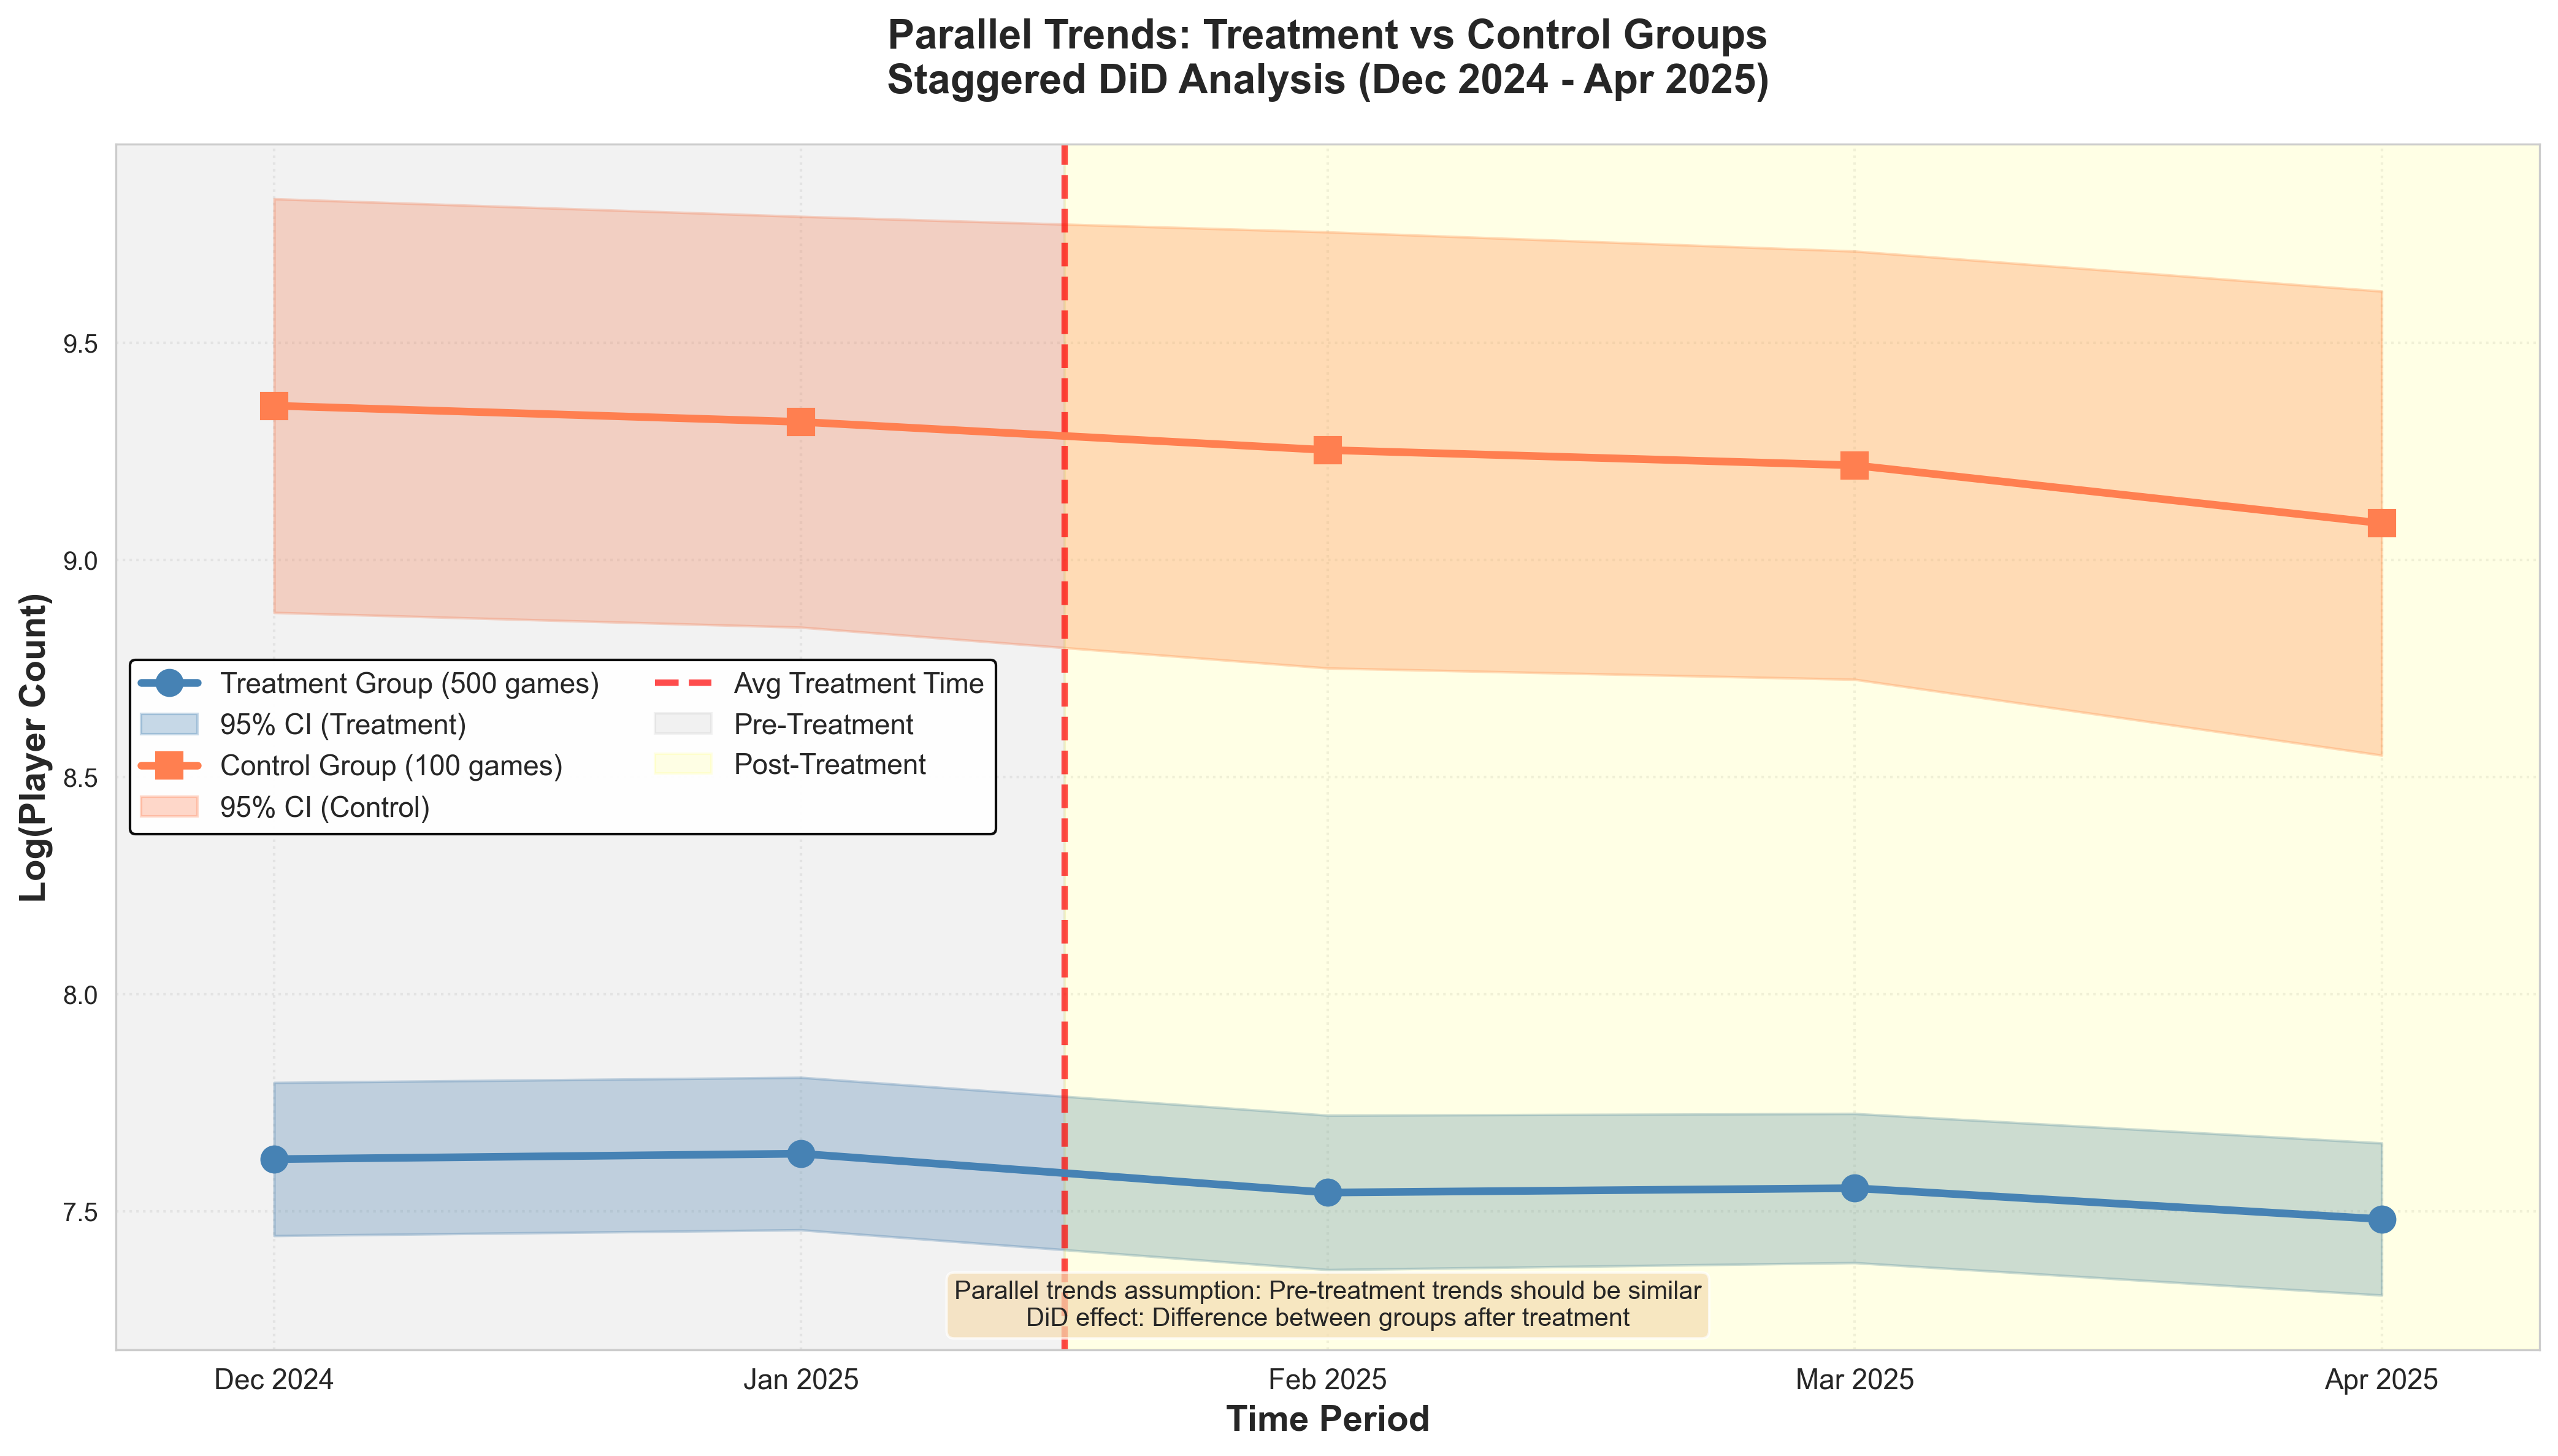
\includegraphics[width=0.8\textwidth]{Actual_final_results/With_Game_FE/staggered_parallel_trends_model2.png}
\caption{Parallel Trends - Staggered Analysis (Model 2)}
\label{fig:parallel_trends}
\end{figure}

\begin{figure}[H]
\centering
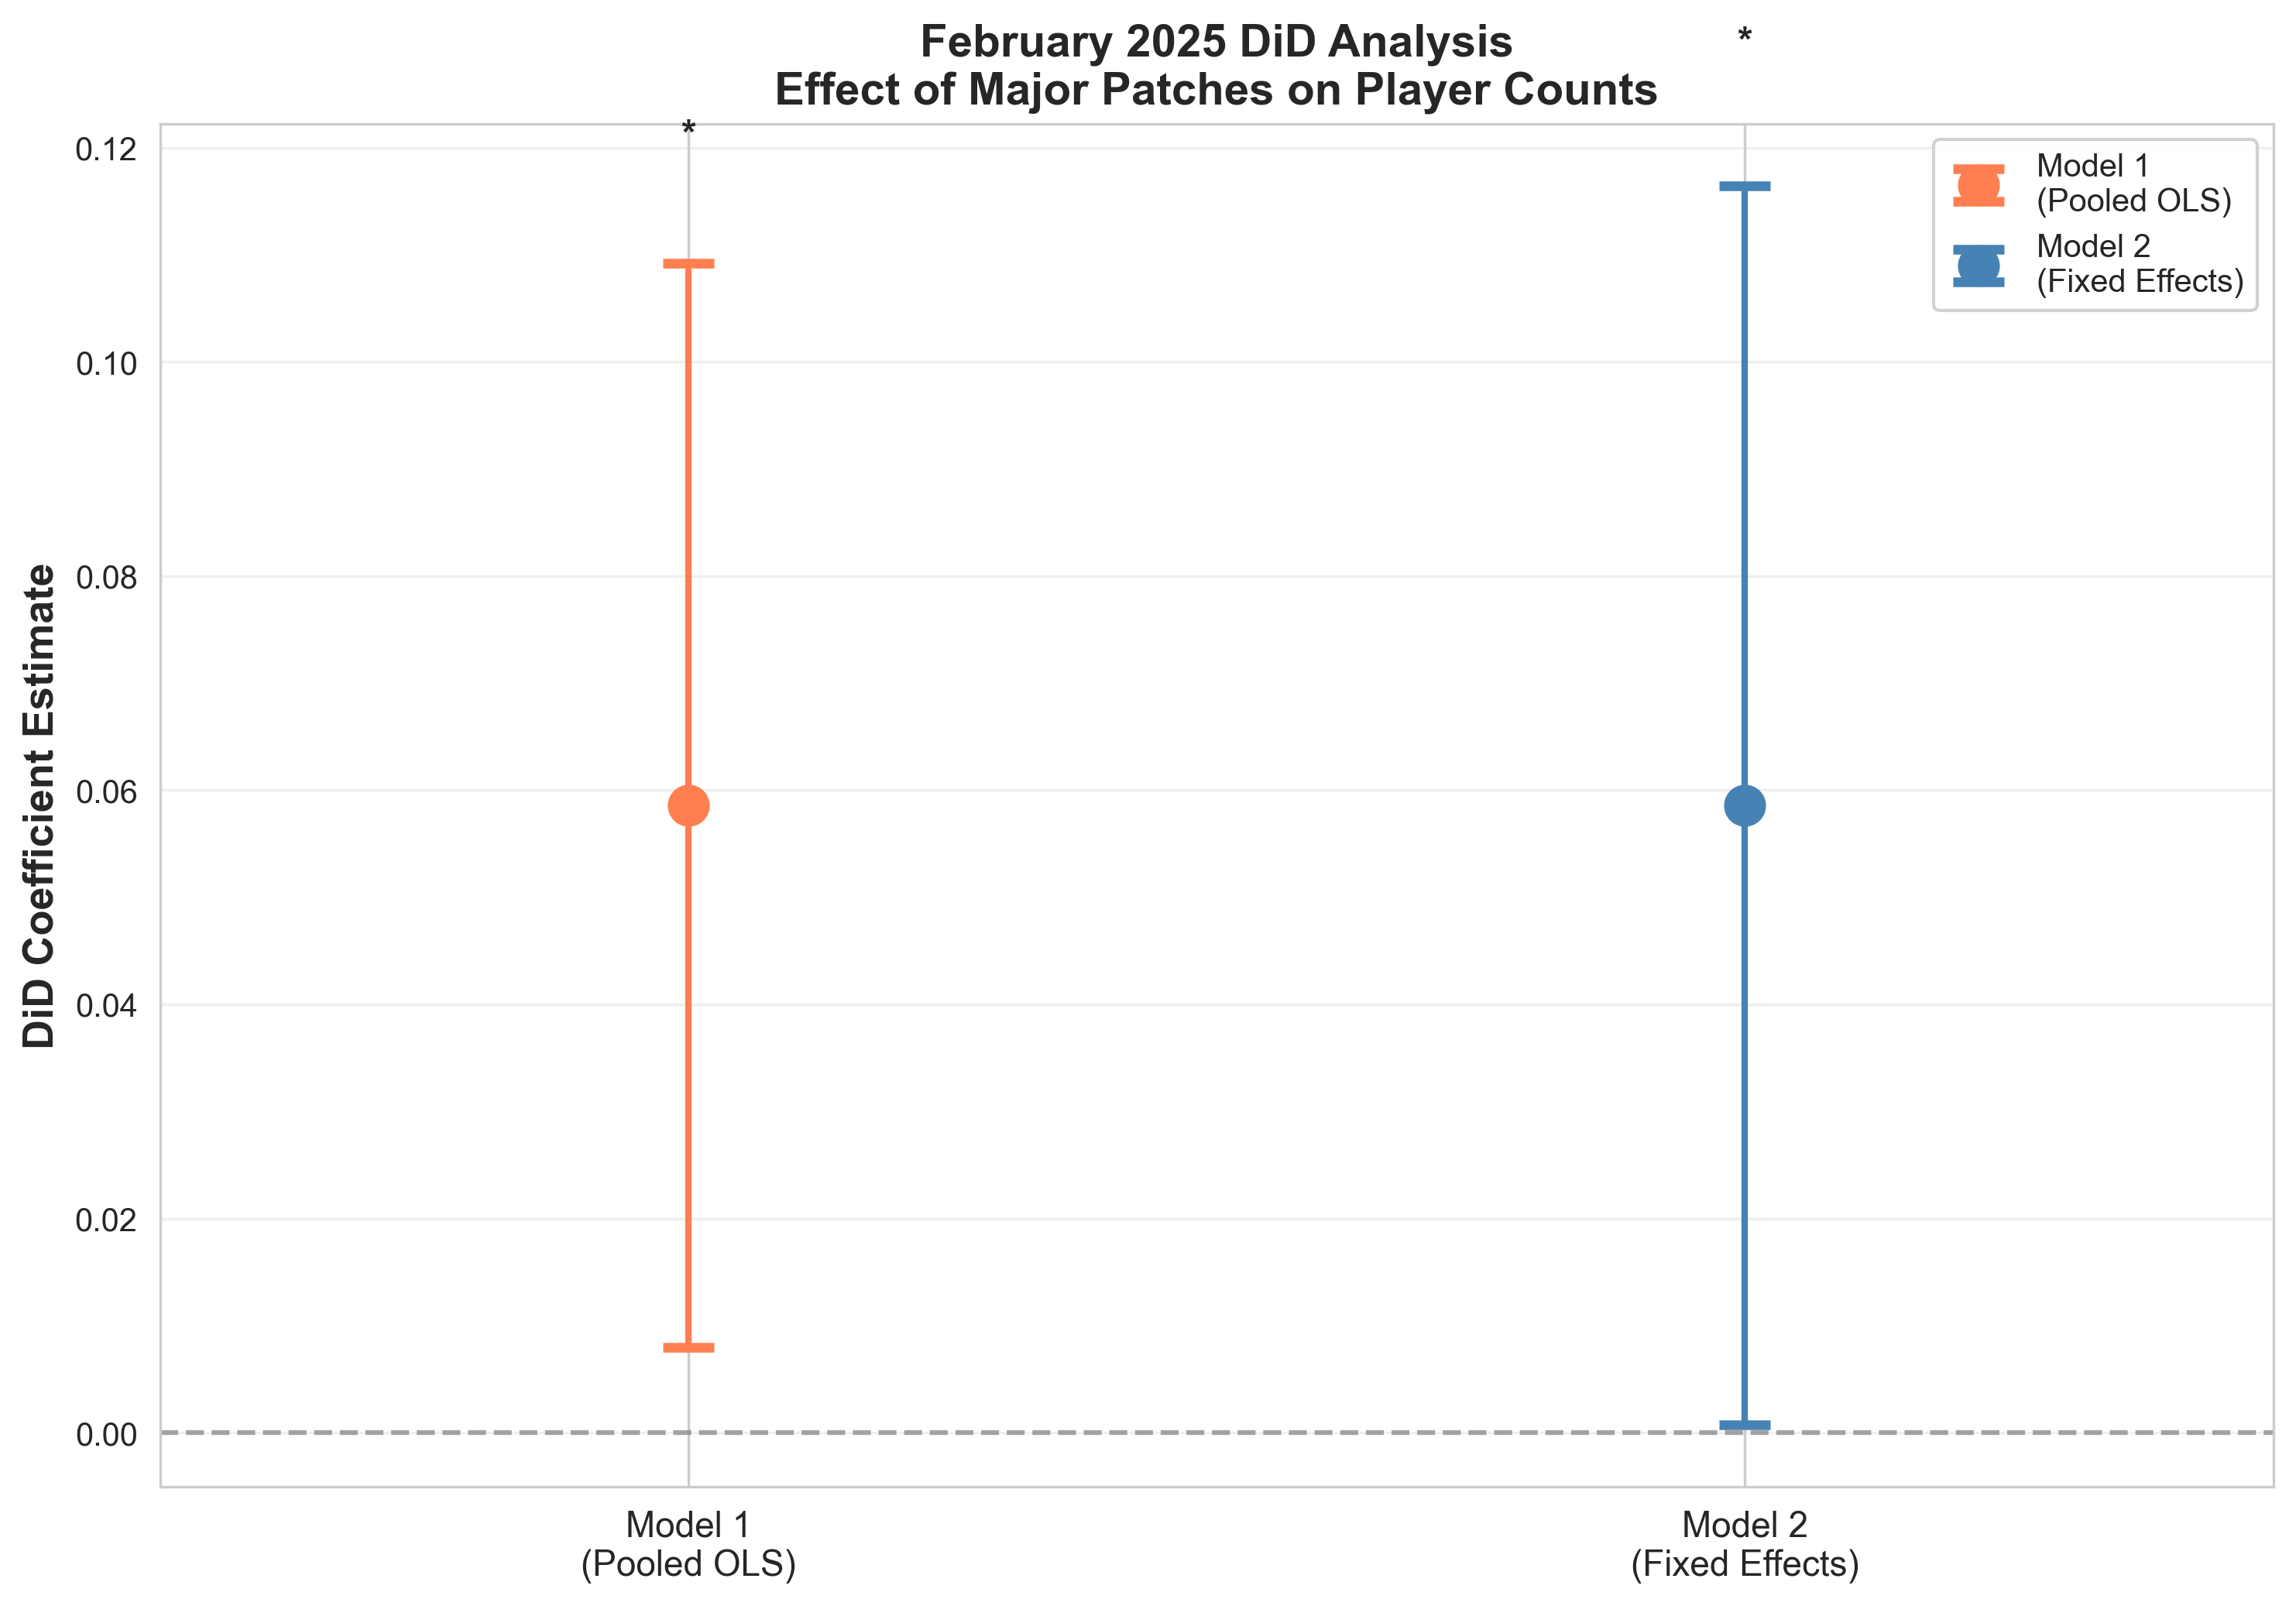
\includegraphics[width=0.8\textwidth]{Actual_final_results/February_only/february_2025_did_coefficient_plot.png}
\caption{DiD Coefficient Estimates - February 2025 Analysis}
\label{fig:february_did}
\end{figure}

\begin{figure}[H]
\centering
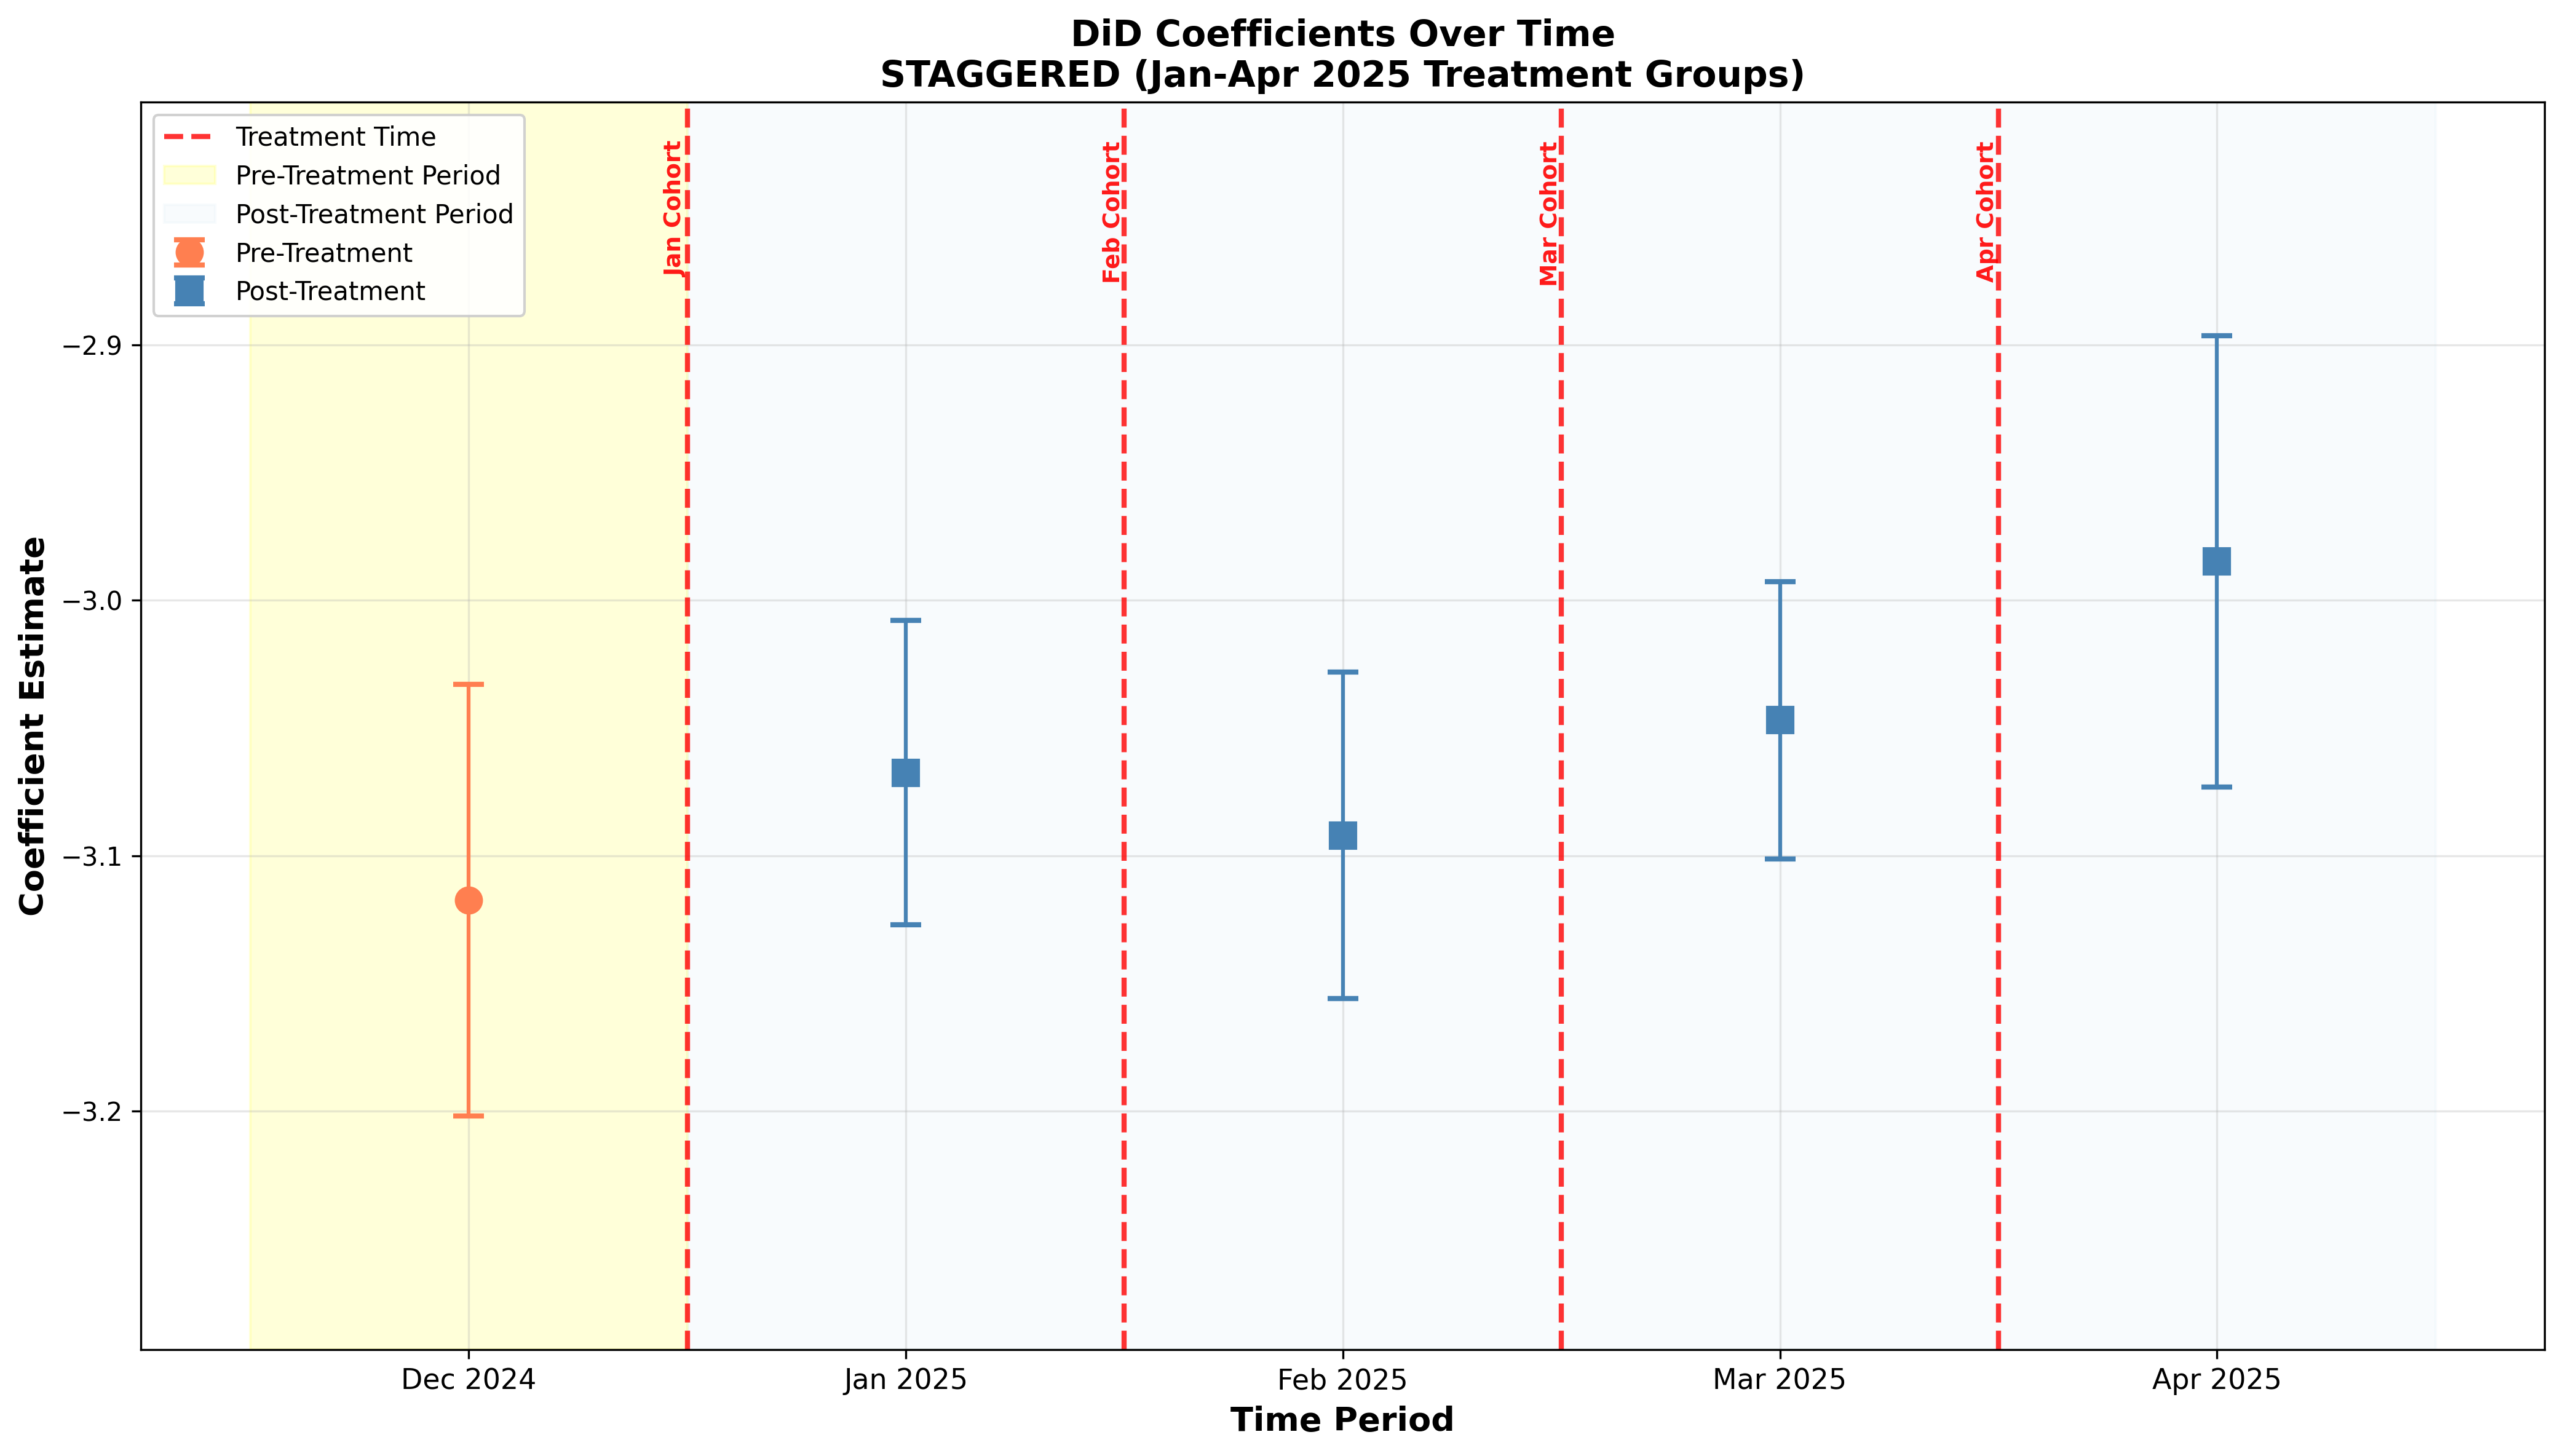
\includegraphics[width=0.8\textwidth]{Actual_final_results/With_Game_FE/staggered_event_study_calendar_time.png}
\caption{Event Study - Staggered Analysis with Treatment Timing Indicators}
\label{fig:event_study}
\end{figure}

\begin{figure}[H]
\centering
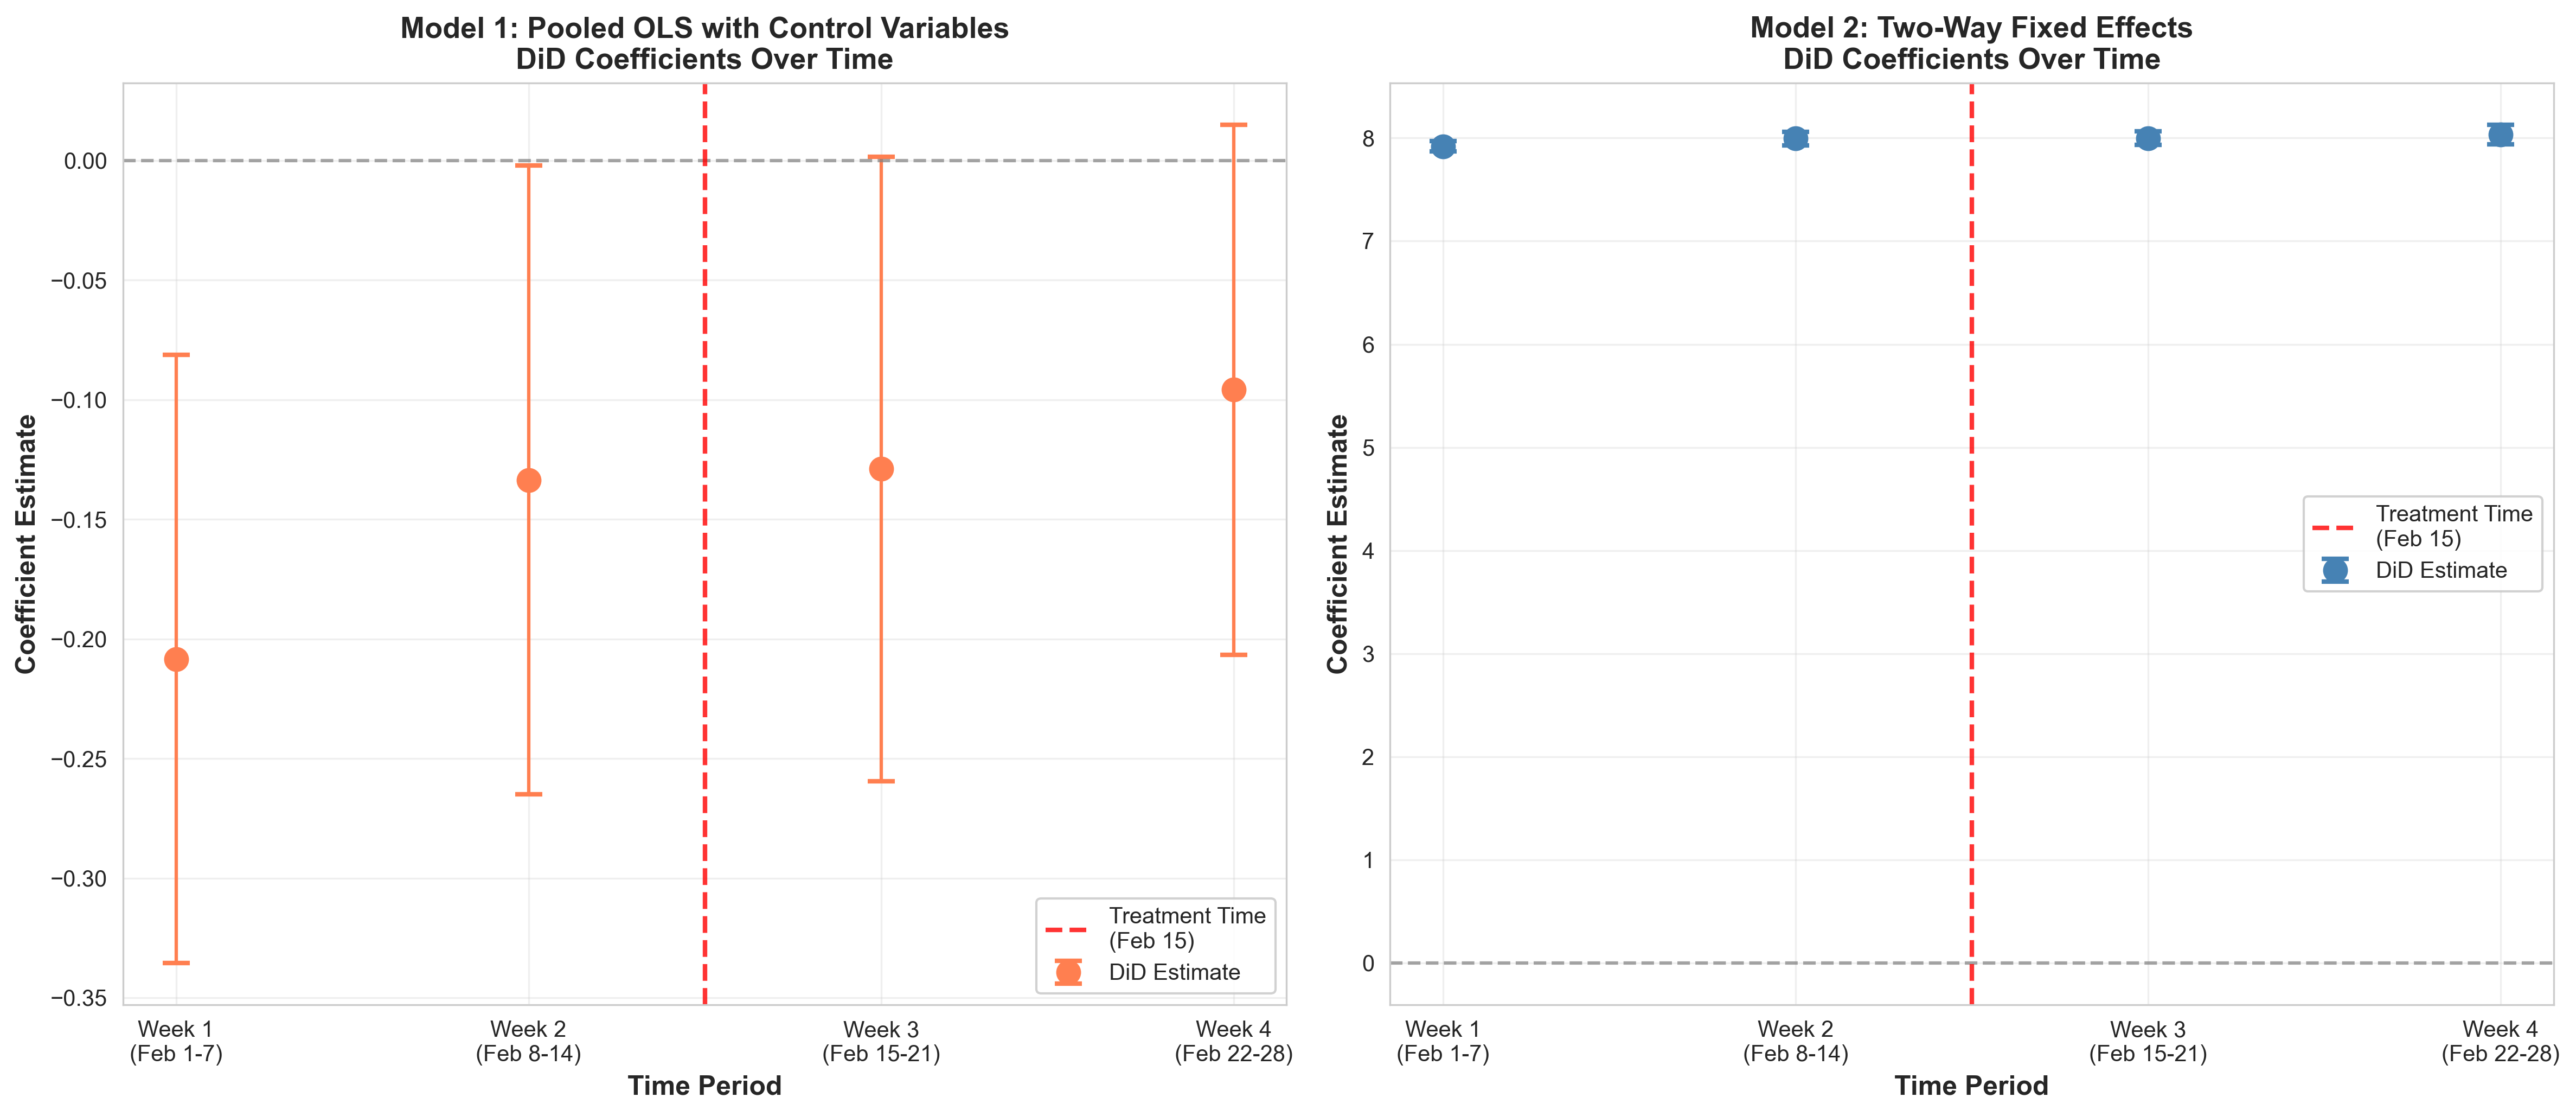
\includegraphics[width=0.8\textwidth]{Actual_final_results/February_only/february_2025_did_coefficients_over_time.png}
\caption{DiD Coefficients Over Time - February 2025 (4 Weeks)}
\label{fig:february_time}
\end{figure}

\section{Conclusion}

\subsection{Main Findings}

This study provides rigorous causal evidence on the impact of major game patches on player engagement in Steam games. Using difference-in-differences methodology with two complementary research designs---a staggered DiD analysis covering 320 games over 5 months and a February 2025 single-cohort analysis of 145 games over 4 weeks---we reach three principal conclusions.

\textbf{First,} major game patches causally increase average concurrent player counts by approximately 6\%. This effect is statistically significant ($p=0.044$ in staggered analysis, $p=0.047$ in February analysis) and remarkably consistent across different samples, time granularities, and observation windows. For a game with 10,000 average concurrent players, this translates to approximately 600 additional players following a major patch release.

\textbf{Second,} naive comparisons that fail to control for selection bias dramatically overestimate treatment effects. Our pooled OLS specification (Model 1) yields an effect size of 41\%, more than six times larger than the true causal estimate of 6\% obtained from our two-way fixed effects specification (Model 2). This 35 percentage point bias arises because games that receive major patches differ systematically from those that do not---likely reflecting differences in developer resources, game quality, and existing player engagement. The fixed effects approach eliminates this bias by controlling for all time-invariant game characteristics and aggregate time shocks.

\textbf{Third,} treatment effects are homogeneous across different patch release timings. Analysis of cohort-specific effects reveals consistent effect sizes (3-8\%) for patches released in January, February, March, and April 2025, with no statistically significant heterogeneity. This suggests that the player engagement response to major patches does not depend critically on seasonal timing within our observation window.

\subsection{Implications for Game Developers}

Our findings carry important implications for game development strategy and post-launch support decisions. While major patches do increase player engagement, the effect is modest in magnitude. Developers should maintain realistic expectations: a 6\% player increase is meaningful but far from transformative. For smaller indie games with limited resources, the cost-benefit calculation of major patch development must account for this modest return.

Moreover, our results highlight that baseline game quality---as measured by review scores---is a far stronger driver of player engagement than post-launch patches. A 10-point improvement in review score predicts a 435\% increase in player counts, dwarfing the 6\% effect of major patches. This suggests that developers should prioritize initial game quality over reactive patching strategies. Patches are valuable for maintaining engagement in already-successful games, but they cannot substitute for fundamental quality.

The consistency of treatment effects across different release timings suggests that developers have flexibility in scheduling major patches without sacrificing effectiveness. There is no evidence that patches released in particular months yield systematically larger player engagement responses.

\subsection{Methodological Contributions}

Beyond substantive findings about patch effects, this study makes several methodological contributions to the analysis of video game markets. We demonstrate the critical importance of controlling for selection bias in observational studies of game updates, showing that naive approaches can overstate effects by an order of magnitude. The two-way fixed effects approach we employ---standard in labor and public economics---merits wider adoption in game industry research.

Our dual research design, combining staggered DiD and single-cohort analyses, provides a template for robustness checking in game analytics. The remarkable consistency of results across these complementary approaches (6.2\% vs 6.0\%) strengthens causal claims and illustrates the value of triangulating evidence from multiple identification strategies.

Finally, we show that SteamCharts data, combined with Steam's public APIs, can support rigorous causal inference for a wide range of research questions in game markets. The data collection pipeline and quality verification procedures we document can be adapted to study other interventions such as sales, content updates, or platform changes.

\subsection{Limitations and Future Research}

Several limitations should inform interpretation of our findings. First, our outcome measure---average concurrent players---captures only one dimension of player engagement. Future research should examine other metrics such as total playtime, session frequency, retention rates, and revenue. Patches may affect these outcomes differently, and the business case for patching depends on revenue impacts that we do not observe.

Second, we treat all ``major patches'' as homogeneous interventions, but patch content varies enormously---from pure bug fixes to expansive new content releases. Future work should distinguish patch types and estimate content-specific effects. We expect that patches adding substantive new features or content yield larger engagement effects than technical updates.

Third, our sample selection process---requiring complete SteamCharts data for all time periods---likely excludes smaller games with minimal player tracking. Results may not generalize to indie games with player counts below SteamCharts' tracking threshold. Moreover, our focus on Steam PC games means findings may not apply to mobile, console, or other gaming platforms with different player dynamics.

Fourth, our observation window is limited to 5 months maximum. We cannot assess whether the measured effects persist over longer horizons or dissipate as players exhaust new content. Longitudinal studies tracking games for 6-12 months post-patch would clarify the durability of treatment effects.

Future research directions include: (1) heterogeneous effects by game genre, distinguishing multiplayer competitive games from single-player narrative games; (2) mechanisms underlying patch effects, separating actual content improvement from media attention and community hype; (3) interaction effects between patches and other marketing activities such as sales or promotions; (4) spillover effects on competing games in the same genre; and (5) optimal patching frequency and timing strategies.

\subsection{Concluding Remarks}

This study provides credible causal evidence that major game patches modestly but significantly increase player engagement in Steam games. The 6\% effect we estimate is policy-relevant for developers making post-launch support decisions, while highlighting that patches alone cannot compensate for fundamental game quality deficits. Methodologically, we demonstrate the severe selection bias present in naive comparisons and the necessity of fixed effects approaches for credible causal inference in observational game data.

As the gaming industry increasingly adopts ``games as a service'' models with continuous post-launch updates, understanding the causal effects of these interventions becomes crucial for strategic planning. Our findings suggest that while patches contribute to player retention, their effects are incremental rather than transformative. Developer resources may be better invested in maximizing initial quality than in reactive patching, though the optimal balance depends on game-specific characteristics and business models that merit further investigation.

\end{document}
